\chapter{Studi Literatur}

Pada bab ini, akan diisi oleh studi literatur, hal-hal yang berkaitan dengan topik persoalan tugas akhir akan dipaparkan dalam bab ini guna untuk memberikan informasi mengenai dasar teori dan studi yang dipakai. Bab ini diharapkan membantu pembaca untuk mengerti dalam membaca penelitian tugas akhir ini.

\section{Sistem Terdistribusi}
\label{sec:sister}

Berdasarkan \parencite{{distributedsystem}, Sistem terdistribusi adalah sistem yang terdiri dari beberapa komputer yang saling terhubung melalui jaringan komputer dan berkomunikasi melalui jaringan tersebut dengan cara bertukar pesan atau \emph{message passing}. Ada beberapa karakteristik dari sistem terdistribusi:

\subsection{\emph{Concurrency}}
Program berjalan secara konkuren pada setiap komputer dalam suatu sistem terdistribusi.

\subsection{\emph{No Global Clock}}
Tidak ada waktu yang akurat dalam suatu sistem terdistribusi. Hal ini diakibatkan oleh adanya waktu yang jumlahnya tidak pasti diperlukan untuk mengirim pesan dalam suatu sistem terdistribusi.

\subsection{\emph{Indepenent Failures}}
Setiap komputer dapat terjadi kegagalan dalam segi program, jaringan, perangkat keras dan sebagainya yang mengakibatkan program yang dijalankan dapat berhenti dimanapun. Maka dari itu, perlu didesain penanganan khusus untuk menanggapi kegagalan dari komputer yang lain pada suatu sistem terdistribusi.

\section{Teorema CAP}

Seperti yang dibahas pada bagian \ref{sec:sister}, ada dua karakteristik yang cukup unik yaitu \emph{concurrency} dan \emph{independent failures}.
Menjalankan beberapa program secara konkuren pada komputer yang sama apabila saling berkegantungan membutuhkan sebuah penanganan khusus apabila program yang lain gagal.
Masalah bertambah ketika program dijalankan secara konkuren pada komputer yang berbeda. Hal-hal yang harus diperhatikan tentunya bertambah seperti masalah jika jaringan terputus, pesan yang dikirimkan hilang, komputer sedang tidak berjalan, dan sebagainya.

Eric Brewer mencetuskan teorema bernama CAP yang sebenarnya merupakan singkatan dari \emph{consistency}, \emph{availability}, dan \emph{Partial tolerance}. Teorema CAP menegaskan bahwa setiap sistem terdistribusi yang menyimpan data dan menggunakan jaringan hanya dapat memiliki dua dari tiga sifat yang diinginkan. Namun, sebenarnya desainer dapat mengoptimalkan komponen konsistensi dan ketersediaan sehingga dapat menimalisir \emph{tradeoff} dari ketiganya \parencite{{captheorem}.

Untuk memilih dua dari tiga sifat yang disebutkan harus ditentukan dari sistem terdistribusi yang dibangun. Terdapat kasus contoh dan penjelasan sebagai berikut.

\subsection{Sistem \emph{Consistency} dan \emph{Availability} (CA)}
Sistem ini mengorbankan partial tolerance. Sehingga, apabila ada suatu komponen dari sistem mati, sistem tidak akan berjalan sama sekali. Pendekatan ini mustahil karena sistem terdistribusi berkaitan dengan komponen yang tersebar di beberapa komputer melalui jaringan. Sangat tidak mungkin untuk mengorbankan komponen \emph{partial tolerance} pada teorema CAP.

\subsection{Sistem \emph{Consistency} dan \emph{Partition Tolerance} (CP)}
Sistem ini biasa digunakan pada sistem yang tidak bisa mengorbankan konsistensi data. Sebagai contoh, pada dunia finansial, data konsisten sangatlah berbahaya. Maka dari itu, banyak sistem perbankan mengorbankan ketersediaan.

\subsection{Sistem \emph{Availability} dan \emph{Partition Tolerance} (AP)}
Sebaliknya, sistem ini mengorbankan faktor konsistensi data. Bukan berarti data tidak pernah konsisten, namun dikenal sebuah istilah \emph{eventually consistent}. Pada sistem yang menggunakan pendekatan AP, kekonsistenan data akan tercapai seiring berjalannya waktu yang berarti komputer-komputer pada sebuah sistem akan berusaha untuk bertukar dan memperbaharui data sehingga pada akhirnya data akan konsisten.

\section{\emph{Microservices}}
\emph{Microservices} adalah layanan yang otonom, berukuran kecil, dan saling bekerja sama dengan \emph{microservice} lainnya. Sebuah \emph{microservice} biasa hidup di dalam sebuah sistem terdistribusi karena sifatnya yang saling membutuhkan layanan lain untuk bekerja sama. Lawan dari \emph{microservice} adalah layanan \emph{monolith}, sebuah layanan yang berukuran besar dan disusun oleh banyak layanan pada layanan yang sama \parencite{{microservice}.

\subsection{Prinsip \emph{Microservice}}
Menurut \parencite{{microservice} terdapat 7 prinsip \emph{microservice}, lihat gambar \ref{fig:prinsip-microservice}.

\begin{figure}[h]
    \centering
    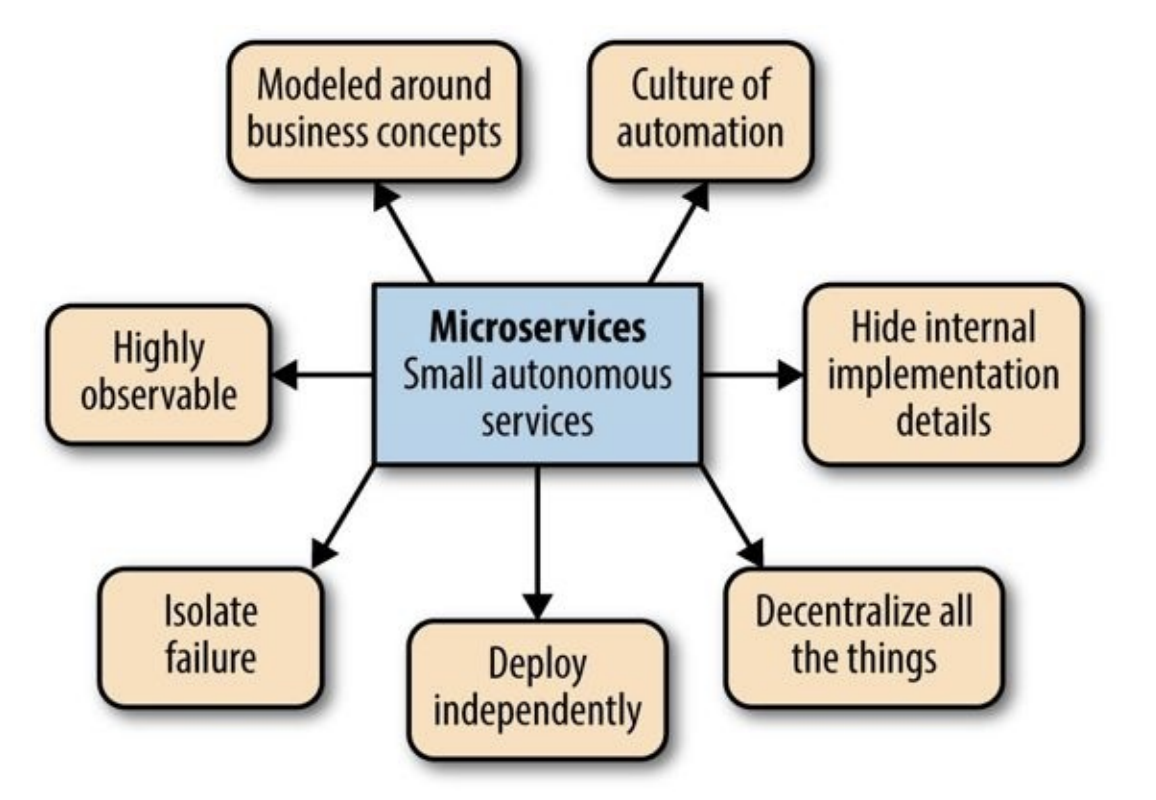
\includegraphics[width=0.8\textwidth]{chapter-2/prinsip-microservice.png}
    \caption{7 Prinsip \emph{Microservice} menurut \parencite{{microservice}}
    \label{fig:prinsip-microservice}
\end{figure}

\subsubsection{\emph{Model Around Business Concepts}}
\emph{Microservice} biasa dimodelkan dekat dengan proses bisnisnya agar bisa menggambarkan konteks pada layanan tersebut. Alasan dimodelkan seperti itu adalah agar layanan lebih stabil dibanding yang dimodelkan dekat dengan konsep teknis.

\subsubsection{\emph{Adopt a Culture of Automation}}
Pembuatan \emph{microservice} menambahkan banyak kompleksitas dalam prosesnya. Untuk mempermudah, diperlukan adanya adopsi terhadap kebiasaan untuk melakukan otomasi. Seperti contohnya melakukan otomasi dalam tahap \emph{deployment} dan \emph{testing} dengan membuat \emph{custom image} yang berisikan variabel \emph{environment} yang sesuai sehingga siap untuk digunakan oleh tim terkait tanpa perlu membutuhkan tim lainnya. 

\subsubsection{\emph{Hide Internal Implementation Details}}
Sebuah \emph{microservice} yang baik tidak mengekspos informasi internal dari layanan itu sendiri. Biasanya basis data yang sama tidak akan digunakan oleh layanan yang berbeda. Layanan yang lain harus meminta dengan mengikuti kontrak dari layanan yang memiliki konteks tersebut.

\subsubsection{\emph{Decentralize All the Things}}
Untuk memaksimalkan \emph{microservice}, diperlukan delegasi pengembangan komponen yang memungkinkan pihak yang bertanggung jawab untuk melakukan pengembangan, pengujian dan \emph{deployment} secara mandiri. Sehingga, tidak dependen kepada tim lain untuk melakukan hal ini.

\subsubsection{\emph{Independently Deployable}}
Layanan juga harus dipastikan bisa di-\emph{deploy} secara mandiri. Bahkan ketika ada perubahan yang dapat merusak, harus dibuat sebuah layanan dengan versi yang berbeda agar pengguna layanan memiliki waktu untuk mengubah dan menyesuaikan.

\subsubsection{\emph{Isolate Failure}}
Sebuah arsitektur \emph{microservice} dikatakan lebih baik daripada arsitektur monolitik saat perancangan kegagalan sudah menjadi bagian dari sistem itu sendiri. Saat membangun komponen-komponennya, harus diperhatikan terhadap partisi jaringan. Entah ketersediaan yang dikorbankan dengan membangun \emph{circuit breaker}, sebuah komponen yang akan menghentikan alur ke sebuah komponen saat kegagalan meningkat, atau mengorbankan konsistensi.

\subsubsection{\emph{Highly Observable}}
Diperlukan juga \emph{monitoring} terhadap layanan-layanan yang ada secara agregat. Tidak mungkin untuk mengandalkan pemantauan terhadap sebuah layanan saja atau mungkin satu mesin saja yang berjalan dengan baik karena \emph{microservice} itu sendiri saling bergantung dengan \emph{microservice} lainnya.

\subsection{Aplikasi 7 Prinsip \emph{Microservice}}
Dengan ketujuh prinsip tersebut, dapat digeneralisir, bahwa layanan \emph{microservice} bersifat independen, terisolasi, dan membutuhkan pendelegasian pekerjaan pada tahap \emph{deployment} serta \emph{testing}. Idealnya, hal tersebut dapat dicapai dengan menjalankan pada lingkungan yang \textbf{terisolasi}. Lingkungan yang \textbf{terisolasi} dapat memudahkan untuk melakukan pemisahan antara suatu \emph{microservice} dengan \emph{microservice} lainnya; memudahkan otomasi \emph{deployment} dan \emph{testing} dengan membuat \emph{image}; memudahkan melakukan pemantauan; dipastikan dapat di-\emph{deploy} secara mandir; dan pastinya menyembunyikan informasi internal. Melakukan isolasi bisa didekatkan dengan virtualisasi dan terdapat dua cara umum untuk melakukan virtualisasi, yaitu dengan \emph{virtual machine} dan \emph{containerization} yang akan dibahas pada bagian \ref{sec:virtualisasi}.


\section{Virtualisasi}
\label{sec:virtualisasi}
\subsection{\emph{Container}}
Seperti namanya, \emph{container} adalah sebuah kontainer yang mengemas aplikasi dengan mengabstraksikan lingkungan aplikasi tersebut. Di dalam kontainer terdapat kode dan \emph{dependencies} dari aplikasi agar dapat dijalankan dengan mudah dan lebih konsisten pada semua lingkungan komputasi \parencite{{containers}.

\subsection{\emph{Virtual Machine}}
\emph{Virtual Machine} melakukan pendekatan virtualisasi dengan mengabstraksikan mulai dari lapisan \emph{hardware stack}. Sehingga, \emph{virtual machine} menempel dengan sistem \emph{hypervisor}. //TODO masih kurang

\subsection{Perbandingan menggunakan \emph{Virtual Machine} dan \emph{Containerization}}
\label{sec:virtualvscontainer}
Sistem \emph{hypervisor} membolehkan mesin dapat menjalankan beberapa sistem operasi tamu jalan di atas sistem operasi utama dengan mengabstraksi sistem komputasi, penyimpanan dan jaringan. Cara kerjanya dengan menggunakan \emph{binary translation} atau \emph{hardware virtualization}. Sedangkan, sebuah \emph{container} merupakan sistem operasi yang lebih ringan yang berjalan di dalam sistem operasi utama dan menjalankan instruksi pada \emph{CPU Core} asli. Sehingga, tidak diperlukannya melakukan translasi atau emulasi instruksi seperti yang dilakukan pada \emph{virtual machine}. Oleh karena itu, \emph{Containerization} lebih menghemat pemakaian sumber daya karena dinilai berhasil menghilangkan \emph{overhead} pada \emph{virtual machine} sambil memberikan sifat isolasi \parencite{{virtualvscontainer}.